\documentclass{article}

% Per-assignment macros
\def\studionumber{7}
\def\studiotitle{Loops}

% Imports
\usepackage{graphicx} % Required for inserting images
\usepackage[colorlinks=true, linkcolor=blue, urlcolor=blue, citecolor=blue, anchorcolor=blue]{hyperref}
\usepackage{hhline}
\usepackage{amsmath}

% Titling
\usepackage{titling}
\preauthor{\begin{center}}
\postauthor{\par\end{center}\vspace{-30pt}}
\setlength{\droptitle}{-50pt}

% Geometry

\usepackage{geometry}
\geometry{letterpaper, portrait, margin=1in}

\usepackage[skip=5pt]{parskip}
\newlength\tindent
\setlength{\tindent}{\parindent}
\setlength{\parindent}{0pt}
\renewcommand{\indent}{\hspace*{\tindent}}

% Assignment titling (number, due date, etc)
\title{
    Studio \studionumber: \studiotitle
}
\author{ENGR 103, Winter 2024}
\date{}

% Box environments
\usepackage{tcolorbox}
\usepackage{fancyvrb}
\newenvironment{terminalcommand}
    {\VerbatimEnvironment
    \begin{tcolorbox}[title=Terminal Command,colframe=gray!80!blue,colback=black!80!blue]
    \begin{Verbatim}[formatcom=\color{white}]}
    {\end{Verbatim}
    \end{tcolorbox}}
\newenvironment{terminaloutput}
    {\VerbatimEnvironment
    \begin{tcolorbox}[title=Terminal Output,colframe=gray!80!red,colback=black!80!blue]
    \begin{Verbatim}[formatcom=\color{white}]}
    {\end{Verbatim}
    \end{tcolorbox}}

\newenvironment{hint}
    {\begin{tcolorbox}[title=Hint,colframe=white!70!blue,colback=white]}
    {\end{tcolorbox}}

\newenvironment{sourcecode}[1]
    {\VerbatimEnvironment
    \begin{tcolorbox}[title=\texttt{#1},colframe=gray!80!green,colback=black!80!blue]
    \begin{Verbatim}[formatcom=\color{white}]}
    {\end{Verbatim}
    \end{tcolorbox}}

\newenvironment{tip}
    {\begin{tcolorbox}[title=Tip,colframe=white!70!blue,colback=white]}
    {\end{tcolorbox}}

\newcounter{examplerun}
\newenvironment{examplerun}
    {\begin{tcolorbox}[title=Example Run \refstepcounter{examplerun}\theexamplerun,colframe=black!50!green,colback=white,subtitle style={boxrule=0.4pt,
colback=lightgray!80!green}]}
    {\end{tcolorbox}}
\newcommand{\exampleruninputs}{\tcbsubtitle{Inputs}}
\newcommand{\examplerunoutputs}{\tcbsubtitle{Outputs}}

\newcounter{exampleproblem}
\newcounter{exampleproblemsolution}
\newenvironment{exampleproblem}
    {\setcounter{exampleproblemsolution}{0}\begin{tcolorbox}[title=Example Problem \refstepcounter{exampleproblem}\theexampleproblem,colframe=black!50!green,colback=white,subtitle style={boxrule=0.4pt,
colback=lightgray!80!green}]}
    {\end{tcolorbox}}
\newcommand{\exampleproblemstatement}{\tcbsubtitle{Problem statement}}
\newcommand{\exampleproblemsolution}{\refstepcounter{exampleproblemsolution}\tcbsubtitle{Solution \theexampleproblemsolution}}

\newcommand{\imagewithdefaults}[1]{\includegraphics[width=\maxwidth{0.95\columnwidth}]{#1}}

\makeatletter
\def\maxwidth#1{\ifdim\Gin@nat@width>#1 #1\else\Gin@nat@width\fi}
\makeatother

\usepackage{soul}

\begin{document}

\maketitle

\section{Loop Problems}

Following are two example problems related to loops. There may be more valid solutions than the ones provided. Make sure you understand them, and then write programs to solve the remaining problems.

\begin{exampleproblem}
    \exampleproblemstatement
    Prompt the user for 10 integers, and then print out the minimum and maximum of all of them. Do not use 10 separate integer variables. Instead, compute the min and max in a running manner.
    
    \exampleproblemsolution
    Notice that this is a ``counting loop'' problem, in the sense that you want to repeat the same instructions a predetermined number of times (10, in this case). A for loop is a good option.
    \\
    \begin{verbatim}
/*
 * Function: prompt_for_number
 * Description: Prompts the user for an integer and returns it
 * Returns (int): Number provided by user
 */
int prompt_for_number() {
    std::cout << "Enter an integer: ";
    int current_num;
    std::cin >> current_num;
}

int main() {
    int max_num;
    int min_num;
    
    for (int i = 0; i < 10; i++) {
        int current_num = prompt_for_number();
    
        if (i == 0 || current_num > max_num) {
            max_num = current_num;
        }
    
        if (i == 0 || current_num < min_num) {
            min_num = current_num;
        }
    }
    
    std::cout << "Max: " << max_num << std::endl;
    std::cout << "Min: " << min_num << std::endl;
}
    \end{verbatim}

    \exampleproblemsolution
    Or, as always, you can simulate the for loop in the previous solution by using a while loop with an external counting variable and a manual increment statement at the end of the loop body (though this wouldn't be as clean).
\end{exampleproblem}

\begin{exampleproblem}
    \exampleproblemstatement
    \begin{enumerate}
        \item \label{int_prompt} Prompt the user for an integer.
        \item Prompt the user for a character that indicates whether they'd like to enter another integer. If the user enters 'Y', then repeat from step \ref{int_prompt}. Otherwise, move on to the next step.
        \item Print the sum of all of the numbers entered by the user.
    \end{enumerate}

    \exampleproblemsolution
    Notice that this program requires executing step 1 \textit{at least once}. A do-while loop is a good option.
    \\
    \begin{verbatim}
/*
 * Same function as in solution to previous problem...
 */
int prompt_for_number() {
    ...
}

/*
 * Function: prompt_for_enter_again
 * Description: Asks the user if they want to enter another number (Y/N)
 * Returns (char): Character entered by user (hopefully Y/N)
 */
char prompt_for_enter_again() {
    char again;
    std::cout << "Would you like to enter another integer?"
        << " Enter Y for yes or N for no: ";
    std::cin >> again;
    return again;
}

int main() {
    char enter_again;
    int sum = 0;
    do {
        int x = prompt_for_number();

        sum += x;

        enter_again = prompt_for_enter_again();
    } while (enter_again == 'Y');
    
    std::cout << "The sum of the integers you entered is: " << sum << std::endl;
}
    \end{verbatim}

    \exampleproblemsolution
    Or, as always, you can simulate the do-while loop in the previous solution using a regular while loop and guaranteeing the loop condition to be true at the start of the loop (though this wouldn't be as clean).
\end{exampleproblem}

\subsection{Problem 1}

Write a program that does the following:

Prompt the user for an integer $N$. Then, prompt the user for $N$ floating point values (i.e., values of type \texttt{double}). Print out the average of all of the $N$ floating point values that the user entered.

\begin{hint}
    An average is computed as $\frac{\text{Sum of values}}{\text{Number of values}}$. In this case, ``Sum of values'' is the sum of all the values entered by the user, and ``Number of values'' is $N$.
\end{hint}

\subsection{Problem 2}

Write a program that does the following:

\begin{enumerate}
    \item Prompt the user for an integer.
    \item Determine whether the entered integer is a prime number. If it is, print ``That number is prime!''. Otherwise, print ``That number is composite!''.
\end{enumerate}

\begin{hint}
    Let $X$ denote the integer in question. $X$ is a prime number if and only if it isn't divisible by any other integers besides $1$ and itself ($X$). For example, $1$, $2$, $3$, $5$, $7$, $11$, $13$, $17$, and $19$ are all prime numbers. $9$ is a composite number (non-prime) because it's divisible by $3$. $15$ is composite because it's divisible by $3$ and $5$. All even numbers besides $2$ are composite because they're all divisible by $2$.

    \vspace{6pt}

    To check if an integer \texttt{a} is divisible by some other integer \texttt{b}, you can use the following boolean expression: \texttt{a \% b == 0}. This expression will evaluate to \texttt{true} if and only if \texttt{a} is divisible by \texttt{b} (make sure you understand why).

    \vspace{6pt}

    Of course, a number can't be divisible by anything larger than it. So your program will only need to check if the user's entered integer is divisible by any other integers smaller than it.
\end{hint}

\subsection{Problem 3}

Write a program that does the following:

Prompt the user for 10 integers. For each integer, compute and print its factorial.

\begin{hint}
    The factorial of $X$ is expressed in mathematics as $x!$ (yes, that exclamation point is a real mathematical operator; it's called the factorial operator).
    
    \vspace{6pt}
    
    A factorial of an integer $X$ is defined as the product of all positive integers that are less than or equal to $X$:

    \vspace{6pt}
    
    $X! = 1 * 2 * 3 * ... * X,$

    \vspace{6pt}

    where $*$ denotes multiplication. You'll need to do this multiplication via a loop.
\end{hint}

\section{Approximating Pi}

\subsection{Context}

\subsubsection{Geometry}

Suppose a unit circle (i.e., a circle with radius 1) is inscribed within a square, like so:

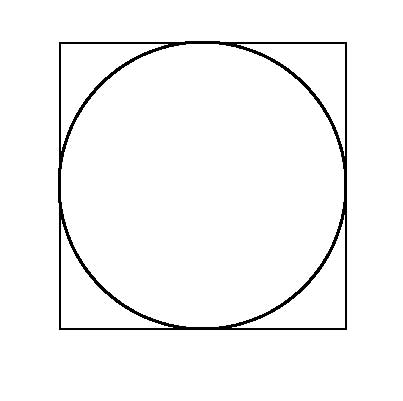
\includegraphics[width=0.5\columnwidth]{res/Circle-inscribed-in-a-square.jpg}

It is known that the area $A$ inside a circle of radius $r$ can be computed as $A = \pi r^2$. Then the area of this particular circle is $A = \pi (1)^2 = \pi$.

Because the radius of the circle is 1, the side length of the square must be 2. Then the area of the square is $2^2 = 4$.

Let $P$ denote the area of the circle divided by the area of the square. In this case, $P = \frac{\pi}{4}$.

Applying algebra, we get $\pi = 4P$. This means that if we can approximate $P$, then we can multiply it by 4 to approximate $\pi$.

\subsubsection{Monte Carlo method}

\href{https://en.wikipedia.org/wiki/Monte_Carlo_method#:~:text=Monte%20Carlo%20methods%2C%20or%20Monte,might%20be%20deterministic%20in%20principle}{Monte Carlo methods} are a class of computational algorithms that use random sampling to form an approximation. Our goal is to approximate $P$, and we're going to do that with a Monte Carlo method.

Consider that if we were to randomly sample Cartesian points within the square, some proportion of them would also land in the circle. In fact, if the sampling distribution is uniform (i.e., every point is equally likely to be sampled), then the probability of a point landing in the circle is exactly equal to $P$. So in order to approximate $P$, all we have to do is sample many points within the square and check what proportion of them landed in the circle.

Let the center of the circle denote the origin $(0, 0)$. Since the square has a side length of 2, the four corners of the square are at coordinates:

\begin{itemize}
    \item -1, 1 (top-left)
    \item 1, 1 (top-right)
    \item 1, -1 (bottom-right)
    \item -1, -1 (bottom-left)
\end{itemize}

To randomly sample a single point within the square, you need to sample an $X$ coordinate within $[-1, 1]$ and a $Y$ coordinate within $[-1, 1]$. Together, they form the sampled point.

A point $(X, Y)$ is within the circle if and only if its distance from the origin is less than or equal to the radius of the circle: $\sqrt{X^2 + Y^2} \leq 1$.

\subsection{Implementation}

Implement the Monte Carlo method described above to approximate $P$. The method says to sample ``many'' points within the square. In this case, sample $100{,}000$ points. Print your approximation of $P$ to standard output. Multiply $P$ by 4 to approximate $\pi$. Print your approximation of $\pi$ to standard output.

\begin{hint}
    Don't sample your coordinates as integers. The truncation would result in a very innacurate approximation. To randomly sample a floating point value (e.g., a \texttt{double}) within some interval $[a, b]$, you can use the following expression: \texttt{(static\_cast<double>(rand()) / RAND\_MAX) * (b - a) + a}
\end{hint}

\end{document}
